\chapter{Por�wnania metod}

W niniejszym rozdziale zostan� por�wnane mi�dzy sob� niekt�re metody.
W celu przeprowadzenia por�wnania dokonano tabelaryzacji najlepszych dla danej metody wynik�w \ref{tabelaporownawcza} oraz przedstawiono je na wykresie por�wnawczym \ref{wykresporownawczy}.

\begin{table}[H]
  \centering
    \begin{tabular}{|c|r|r|r|r|r|r|}
    \hline
    \multirow{2}[4]{*}{\textbf{Sekwencja}} & \multicolumn{6}{c|}{\textbf{Metoda}} \bigstrut\\
\cline{2-7}          & \multicolumn{1}{c|}{\textbf{�rednia}} & \multicolumn{1}{c|}{\textbf{Mediana}} & \multicolumn{1}{c|}{\textbf{MOG}} & \multicolumn{1}{c|}{\textbf{\parbox[top][2cm][c]{2.3cm}{Aproksymacja �redniej}}} & \multicolumn{1}{c|}{\textbf{DCT}} & \multicolumn{1}{c|}{\textbf{Hadamard}} \bigstrut\\
    \hline
    \textbf{clip\_01.mpg} & 85.9989 & 53.8921 & 86.2640 & 64.5492 & 43.1881 & 43.1868 \bigstrut\\
    \hline
    \textbf{clip\_02.mpg} & 38.3934 & 13.1536 & 25.1933 & 29.5430 & 37.5261 & 37.5051 \bigstrut\\
    \hline
    \textbf{clip\_03.mpg} & 198.5494 & 201.5418 & 181.0108 & 151.6200 & 183.3507 & 183.3458 \bigstrut\\
    \hline
    \textbf{clip\_04.mpg} & 62.8719 & 32.7241 & 63.4837 & 21.6948 & 34.1747 & 34.3609 \bigstrut\\
    \hline
    \textbf{fountain.mpg} & 37.7537 & 36.5344 & 29.1133 & 13.0922 & 70.7695 & 70.7736 \bigstrut\\
    \hline
    \textbf{highway.mpg} & 56.4986 & 52.7896 & 55.6217 & 71.3761 & 47.3152 & 47.8593 \bigstrut\\
    \hline
    \textbf{pedestrians.mpg} & 105.0423 & 24.9158 & 33.3411 & 67.8489 & 84.5606 & 84.5457 \bigstrut\\
    \hline
    \end{tabular}%
\caption{Wykres por�wnawczy wszystkich metod}
\label{tabelaporownawcza}
\end{table}%



\begin{figure}[H]
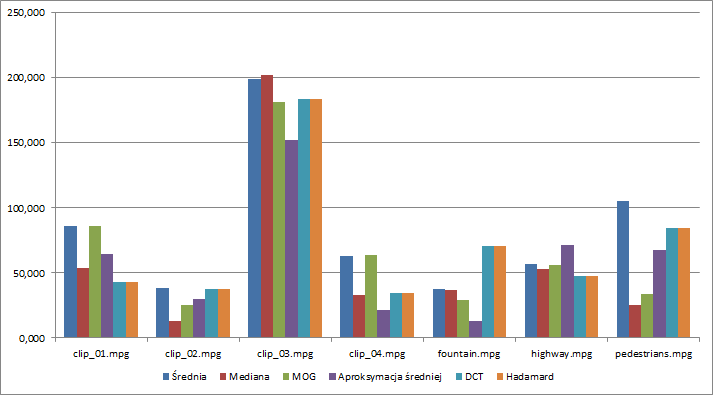
\includegraphics[width=\textwidth]{wszyetkiewykres.PNG}
\caption{Wykres por�wnawczy wszystkich metod}
\label{wykresporownawczy}
\end{figure}
\section{Por�wnanie metody MOG z metod� mediany z bufora}

% Table generated by Excel2LaTeX from sheet 'Sheet1'
\begin{table}[htbp]
  \centering
    \begin{tabular}{|r|r|r|}
    \hline
    \multicolumn{1}{|c|}{\multirow{2}[4]{*}{\textbf{Sekwencja}}} & \multicolumn{2}{c|}{\textbf{Metoda}} \bigstrut\\
\cline{2-3}    \multicolumn{1}{|c|}{} & \textbf{Mediana} & \textbf{MOG} \bigstrut\\
    \hline
    \textbf{clip\_01.mpg} & 53,8921 & 86,2640 \bigstrut\\
    \hline
    \textbf{clip\_02.mpg} & 13,1536 & 25,1933 \bigstrut\\
    \hline
    \textbf{clip\_03.mpg} & 201,5418 & 181,0108 \bigstrut\\
    \hline
    \textbf{clip\_04.mpg} & 32,7241 & 63,4837 \bigstrut\\
    \hline
    \textbf{fountain.mpg} & 36,5344 & 29,1133 \bigstrut\\
    \hline
    \textbf{highway.mpg} & 52,7896 & 55,6217 \bigstrut\\
    \hline
    \textbf{pedestrians.mpg} & 24,9158 & 33,3411 \bigstrut\\
    \hline
    \end{tabular}%
\caption{Tabela por�wnawcza metod MOG i mediany z bufora}
\label{MOGMEDporownanietabela}
\end{table}%

\begin{figure}[H]
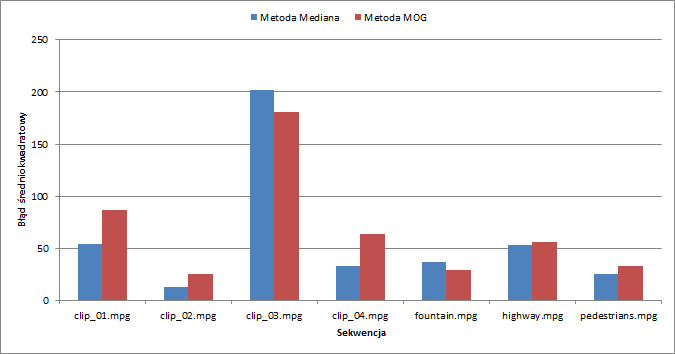
\includegraphics[width=\textwidth]{MOGMED.PNG}
\caption{Wykres por�wnawczy metody MOG z metod� mediany z bufora}
\label{wykresporownawczyMOGMED}
\end{figure}
